\chapter{代码}

\section{行人导航系统伪代码}

\renewcommand{\thealgorithm}{A.\arabic{algorithm}}

\begin{algorithm}[H]
\caption{Carla行人导航系统主流程}
\begin{algorithmic}[1]
\STATE 启动GUI窗口,初始化控件与信号连接
\STATE 点击“初始化环境”时:
    \STATE \quad 连接Carla服务器,加载Town01地图
    \STATE \quad 解析CSV文件构建k近邻导航图,检测最大连通子图
    \STATE \quad 筛选有效生成点并设置SpinBox编号范围
\STATE 点击“开始训练”时:
    \STATE \quad 获取训练参数(学习率、GAE λ、熵系数等)
    \STATE \quad 创建训练线程 \texttt{TrainingThread},初始化PPO模型
    \STATE \quad 每n\_steps同步训练进度,每50 episode保存检查点
\STATE 点击“运行演示”时:
    \STATE \quad 加载预训练模型,基于A*路径执行导航
    \STATE \quad 实时绘制轨迹点与规划路径箭头
\STATE 进入主事件循环,处理可视化工具操作与线程控制
\end{algorithmic}
\end{algorithm}

\begin{algorithm}[H]
\caption{环境类 \texttt{EnhancedPedestrianEnv} 核心结构}
\begin{algorithmic}[1]
\STATE 初始化:连接Carla服务器,构建可行走点导航图
\STATE 筛选有效生成点(验证Spawn点可生成性)
\STATE 定义动作空间(5维离散动作),观察空间(12维状态向量):
    \STATE \quad 归一化位置、目标方向、障碍距离、路径偏离等
\STATE 每步执行:
    \STATE \quad 解析动作(转向角+速度比),计算安全速度
    \STATE \quad 基于目标方向自动调整偏航角
    \STATE \quad 应用行人控制并更新轨迹可视化
    \STATE \quad 计算奖励:目标接近奖励 + 路径跟随奖励 - 碰撞惩罚
    \STATE \quad 激光雷达障碍检测(最小距离更新)
\STATE 路径规划:
    \STATE \quad 基于CSV导航点构建图结构,执行A*搜索
    \STATE \quad 合法性检查(起点/终点在最大连通子图中)
\STATE 重置环境时清理旧Actor,重新生成传感器与标记
\end{algorithmic}
\end{algorithm}

\begin{algorithm}[H]
\caption{训练线程 \texttt{TrainingThread} 流程}
\begin{algorithmic}[1]
\REQUIRE 环境参数(起止点编号、摄像头跟随标志)
\REQUIRE 训练参数(n\_steps=4096, batch\_size=256, total\_steps=1e5)
\STATE 初始化向量化环境 \texttt{DummyVecEnv}
\STATE 配置PPO策略网络(双128层ReLU网络)
\STATE for $step \leftarrow 0$ to \texttt{total\_steps} by \texttt{n\_steps} do
    \STATE 执行策略rollout收集经验数据
    \STATE 计算GAE优势估计,更新策略参数
    \STATE 同步训练进度至GUI(奖励曲线、进度条)
    \IF{episode\_count \% 50 == 0}
        \STATE 保存检查点(时间戳命名)
    \ENDIF
\STATE 保存最终模型,释放GPU显存
\end{algorithmic}
\end{algorithm}

\begin{algorithm}[H]
\caption{导航图构建与路径规划}
\begin{algorithmic}[1]
\REQUIRE CSV可行走点文件(x,y,z,index)
\STATE 加载CSV点集,构建无向图G
\STATE for each point $p_i$:
    \STATE \quad 查找k个最近邻点,添加带权边(距离为权重)
\STATE 提取最大连通子图,缓存合法节点索引
\STATE 路径搜索:
    \STATE \quad 查找起点/终点最近图节点
    \STATE \quad 执行A*算法(启发函数为欧氏距离)
    \STATE \quad 路径合法性验证(节点在连通子图中)
\STATE 返回路径点列表,转换为Dummy Waypoint格式
\end{algorithmic}
\end{algorithm}


% 用户手册章节
\chapter{用户手册}

\section{Carla 行人导航系统使用指南}

\begin{table}[H]
\centering
\renewcommand{\arraystretch}{1.3}
\begin{tabular}{
  >{\centering\arraybackslash}p{3cm}
  >{\centering\arraybackslash}p{8cm}
  >{\centering\arraybackslash}p{4cm}
}
\toprule
\textbf{版本号} & \textbf{描述} & \textbf{日期} \\
\midrule
v1.4.0 & 新增导航图连通性分析、路径合法性检测、PyQt6界面升级 & 2025年5月17日 \\
\bottomrule
\end{tabular}
\caption{系统版本信息}
\label{tab:version-info}
\end{table}

\subsection{系统简介}
本系统基于Carla 0.9.15与PyQt6框架,集成以下创新特性:
\begin{itemize}
\item 基于CSV可行走点构建k近邻导航图,支持最大连通子图提取
\item 增强路径合法性检测机制,自动提示不可达路径
\item 动态轨迹可视化(绿色轨迹点 + 红色路径箭头)
\item 多线程训练架构,支持CUDA加速与模型检查点保存
\end{itemize}

\subsection{配置要求}
\subsubsection*{硬件配置}
\begin{itemize}
\item GPU:支持CUDA 11.7+(需8GB显存)
\item 内存:16GB DDR4(训练时建议32GB)
\end{itemize}

\subsubsection*{软件依赖}
\begin{itemize}
\item \texttt{PyQt6}取代PyQt5,需通过pip安装:
\begin{lstlisting}[language=bash]
pip install pyqt6 carla gymnasium stable-baselines3
\end{lstlisting}
\item Carla PythonAPI需与服务器版本匹配(0.9.15)
\end{itemize}

\subsection{GUI模块详解}
\begin{figure}[H]
\centering
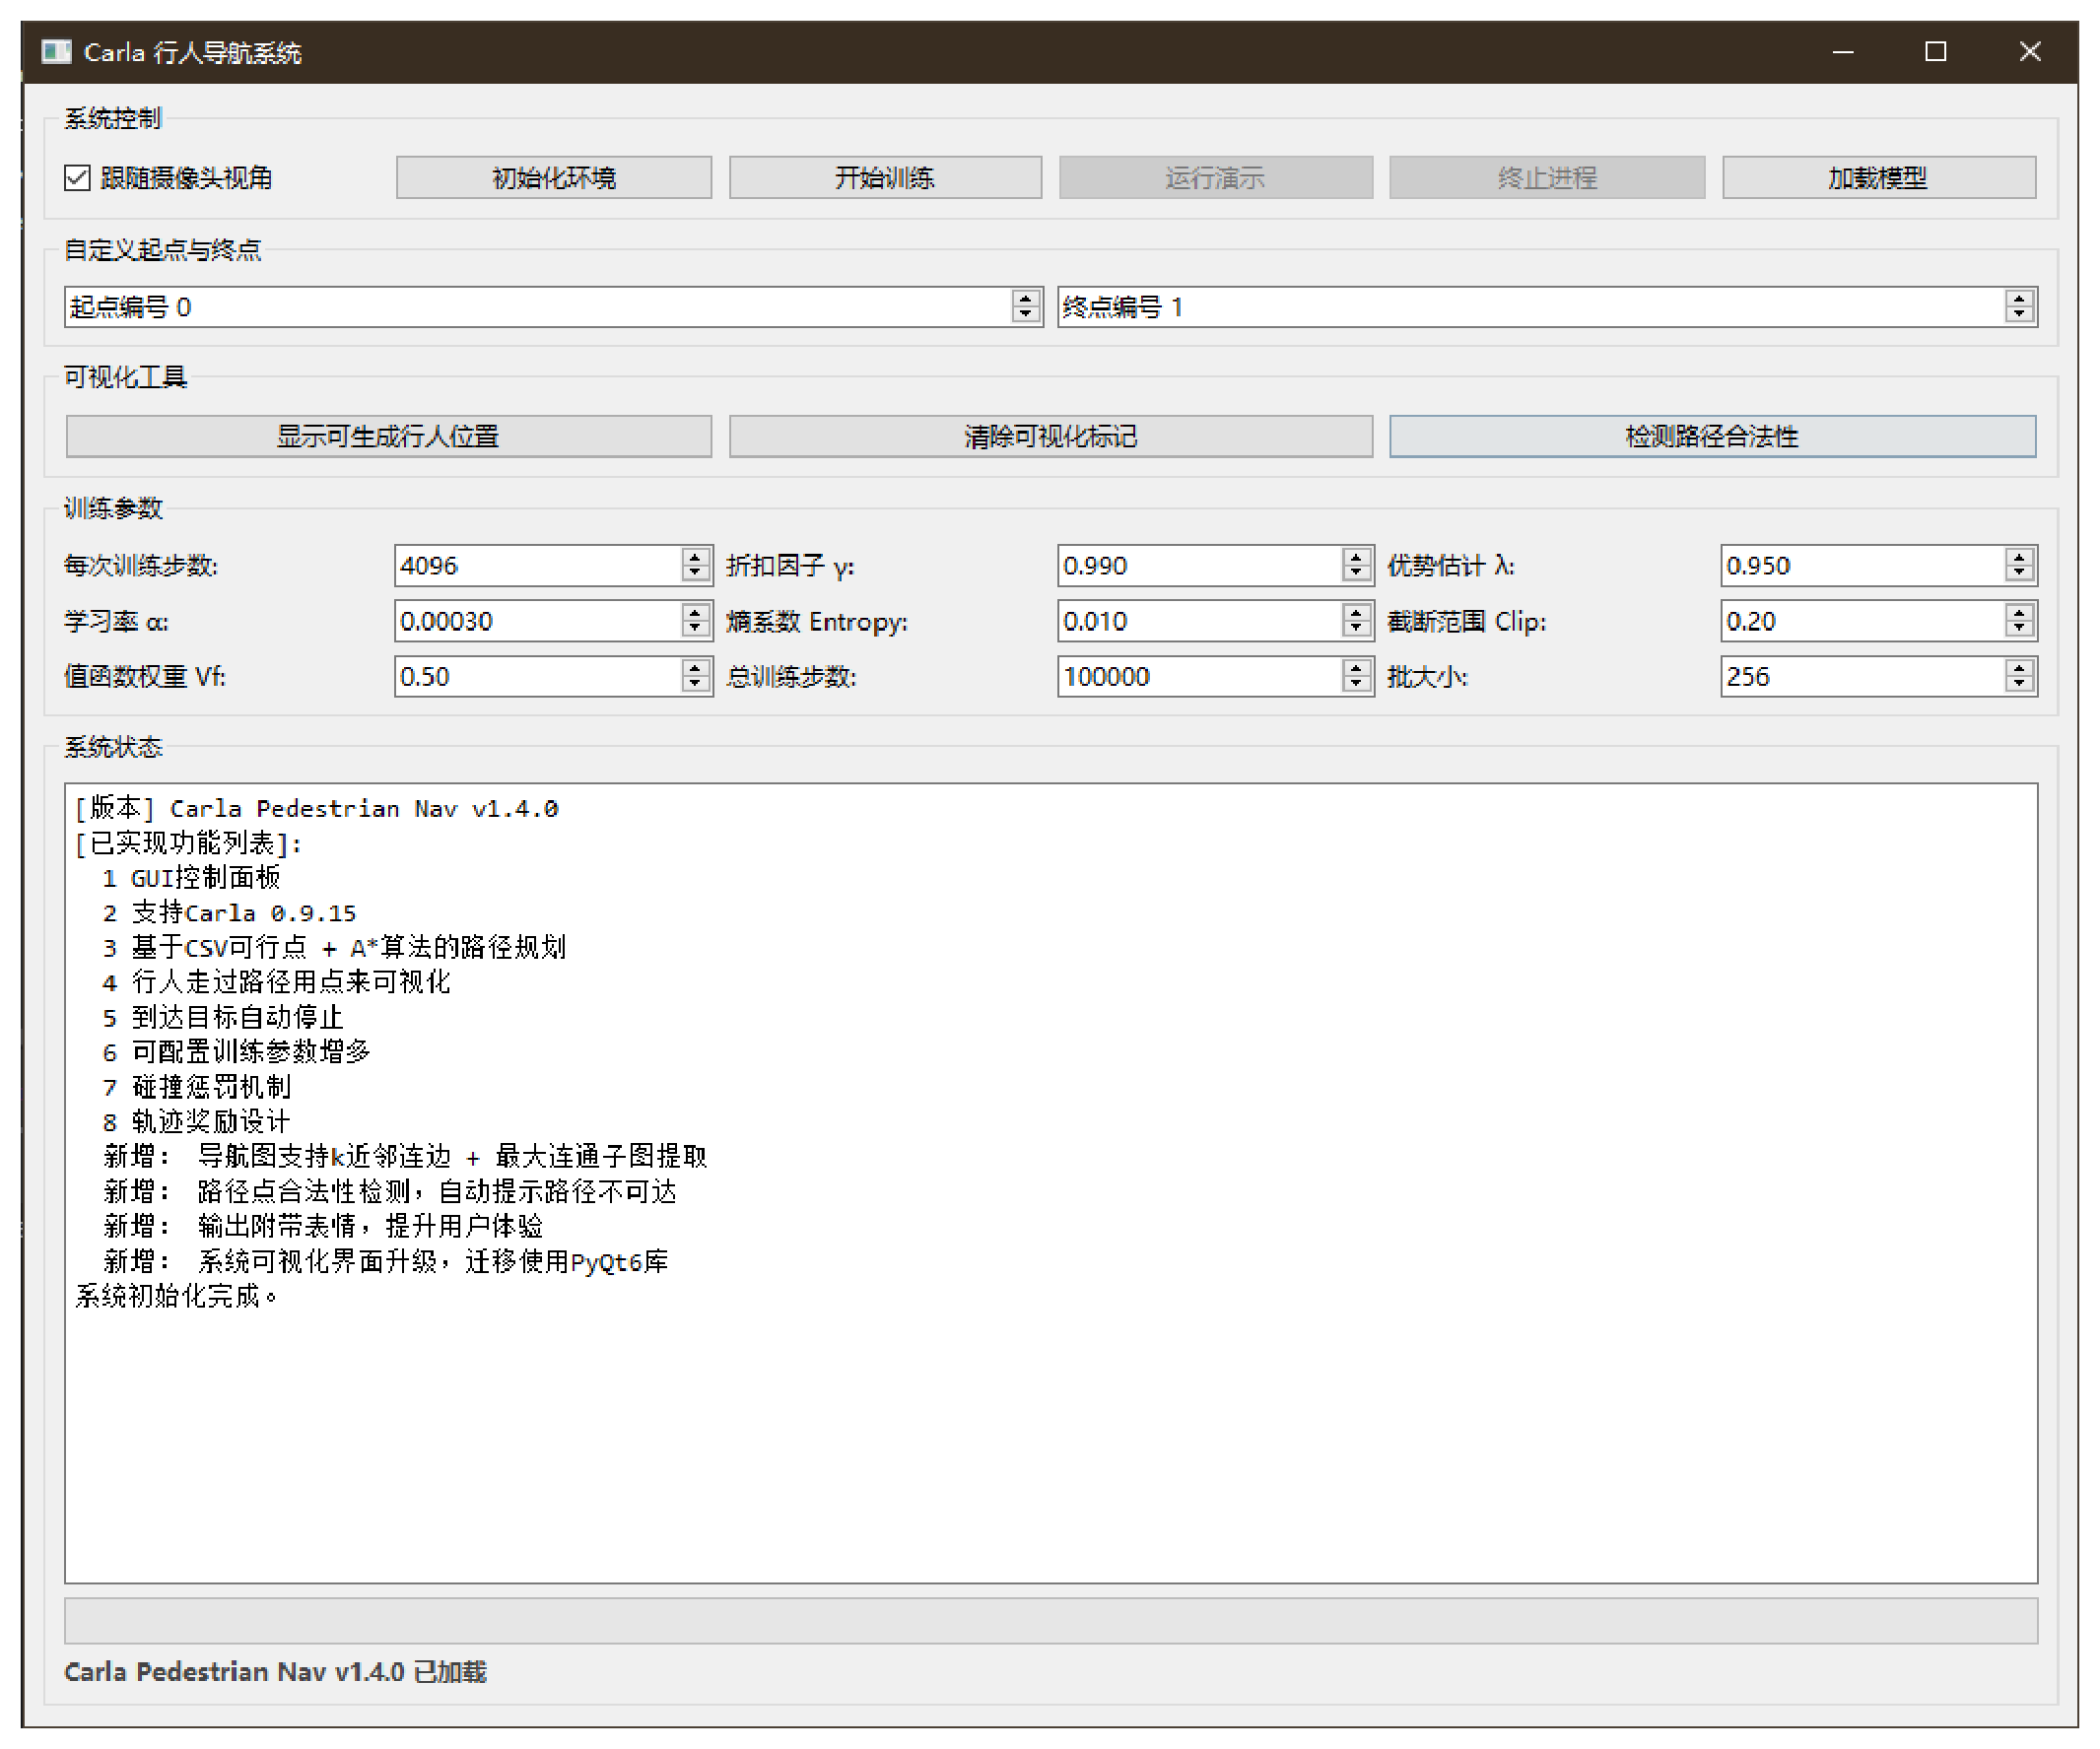
\includegraphics[width=1\textwidth]{images/gui_layout.pdf}
\caption{GUI界面功能分区示意图}
\label{fig:gui-layout}
\end{figure}

\subsubsection*{新增功能控件}
\begin{itemize}
\item 路径合法性检测:点击后扫描CSV文件,输出可达路径对
\item 清除调试标记:一键清除Carla世界中的所有可视化对象
\item 摄像头视角跟随:勾选后第三人称视角跟踪行人移动
\end{itemize}

\subsection{训练参数优化建议}
\begin{table}[H]
\centering
\renewcommand{\arraystretch}{1.2}
\caption{关键参数经验值}
\begin{tabular}{lll}
\toprule
\textbf{参数} & \textbf{推荐值} & \textbf{作用} \\
\midrule
k近邻数 & 6 & 平衡图连通性与计算效率 \\
路径偏离半径 & 2.0m & 控制路径跟随奖励的阈值 \\
同步模式帧率 & 50FPS & 保证传感器数据时序一致性 \\
目标容差 & 1.5m & 判定到达目标的距离阈值 \\
\bottomrule
\end{tabular}
\end{table}

\subsection{典型工作流程}
\begin{enumerate}
\item \textbf{环境预配置}:
    \begin{lstlisting}[language=bash]
    # 生成可行走点CSV(需提前运行)
    python generate_walkable_points.py --town Town01
    \end{lstlisting}
\item \textbf{训练阶段}:
    \begin{itemize}
    \item 设置起点/终点编号跨度>50以保证路径复杂度
    \item 首次训练建议启用"摄像头跟随"以实时观察策略表现
    \end{itemize}
\item \textbf{演示阶段}:
    \begin{itemize}
    \item 加载模型后点击"显示可行走点"验证起终点位置
    \item 路径异常时可点击"清除标记"重新规划
    \end{itemize}
\end{enumerate}

\begin{table}[H]
\centering
\renewcommand{\arraystretch}{1.3}
\caption{增强版故障排查指南}
\begin{tabular}{
  >{\centering\arraybackslash}p{6cm}
  >{\centering\arraybackslash}p{9cm}
}
\toprule
\textbf{现象} & \textbf{解决方案} \\
\midrule
A*路径搜索失败 & 检查CSV文件完整性,确保起终点在最大连通子图内 \\
激光雷达无数据 & 验证行人高度是否>2m(z=2.5的安装位置) \\
训练时奖励震荡 & 降低学习率至1e-5,增加batch\_size至512 \\
GUI线程卡死 & 避免在训练过程中操作SpinBox控件 \\
\bottomrule
\end{tabular}
\end{table}

\subsection{开发者扩展接口}
\begin{itemize}
\item 自定义路径规划算法:
\begin{lstlisting}[language=Python]
def _generate_path(self):
    # 重写此方法实现RRT等算法
\end{lstlisting}
\item 增加观测维度:
\begin{lstlisting}[language=Python]
# 修改observation_space与_get_obs()
self.observation_space = spaces.Box(...) 
\end{lstlisting}
\item 添加新传感器:
\begin{lstlisting}[language=Python]
def _attach_sensors(self):
    # 参照_lidar配置新增RGB相机等
\end{lstlisting}
\end{itemize}
